%% LaTeX Beamer presentation template (requires beamer package)
%% see http://latex-beamer.sourceforge.net/
%% idea contributed by H. Turgut Uyar
%% template based on a template by Till Tantau
%% this template is still evolving - it might differ in future releases!

\documentclass[xcolor=svgnames]{beamer} 

%% ODER: format ==         = "\mathrel{==}"
%% ODER: format /=         = "\neq "
%
%
\makeatletter
\@ifundefined{lhs2tex.lhs2tex.sty.read}%
  {\@namedef{lhs2tex.lhs2tex.sty.read}{}%
   \newcommand\SkipToFmtEnd{}%
   \newcommand\EndFmtInput{}%
   \long\def\SkipToFmtEnd#1\EndFmtInput{}%
  }\SkipToFmtEnd

\newcommand\ReadOnlyOnce[1]{\@ifundefined{#1}{\@namedef{#1}{}}\SkipToFmtEnd}
\usepackage{amstext}
\usepackage{amssymb}
\usepackage{stmaryrd}
\DeclareFontFamily{OT1}{cmtex}{}
\DeclareFontShape{OT1}{cmtex}{m}{n}
  {<5><6><7><8>cmtex8
   <9>cmtex9
   <10><10.95><12><14.4><17.28><20.74><24.88>cmtex10}{}
\DeclareFontShape{OT1}{cmtex}{m}{it}
  {<-> ssub * cmtt/m/it}{}
\newcommand{\texfamily}{\fontfamily{cmtex}\selectfont}
\DeclareFontShape{OT1}{cmtt}{bx}{n}
  {<5><6><7><8>cmtt8
   <9>cmbtt9
   <10><10.95><12><14.4><17.28><20.74><24.88>cmbtt10}{}
\DeclareFontShape{OT1}{cmtex}{bx}{n}
  {<-> ssub * cmtt/bx/n}{}
\newcommand{\tex}[1]{\text{\texfamily#1}}	% NEU

\newcommand{\Sp}{\hskip.33334em\relax}


\newcommand{\Conid}[1]{\mathit{#1}}
\newcommand{\Varid}[1]{\mathit{#1}}
\newcommand{\anonymous}{\kern0.06em \vbox{\hrule\@width.5em}}
\newcommand{\plus}{\mathbin{+\!\!\!+}}
\newcommand{\bind}{\mathbin{>\!\!\!>\mkern-6.7mu=}}
\newcommand{\sequ}{\mathbin{>\!\!\!>}}
\renewcommand{\leq}{\leqslant}
\renewcommand{\geq}{\geqslant}
\usepackage{polytable}

%mathindent has to be defined
\@ifundefined{mathindent}%
  {\newdimen\mathindent\mathindent\leftmargini}%
  {}%

\def\resethooks{%
  \global\let\SaveRestoreHook\empty
  \global\let\ColumnHook\empty}
\newcommand*{\savecolumns}[1][default]%
  {\g@addto@macro\SaveRestoreHook{\savecolumns[#1]}}
\newcommand*{\restorecolumns}[1][default]%
  {\g@addto@macro\SaveRestoreHook{\restorecolumns[#1]}}
\newcommand*{\aligncolumn}[2]%
  {\g@addto@macro\ColumnHook{\column{#1}{#2}}}

\resethooks

\newcommand{\onelinecommentchars}{\quad-{}- }
\newcommand{\commentbeginchars}{\enskip\{-}
\newcommand{\commentendchars}{-\}\enskip}

\newcommand{\visiblecomments}{%
  \let\onelinecomment=\onelinecommentchars
  \let\commentbegin=\commentbeginchars
  \let\commentend=\commentendchars}

\newcommand{\invisiblecomments}{%
  \let\onelinecomment=\empty
  \let\commentbegin=\empty
  \let\commentend=\empty}

\visiblecomments

\newlength{\blanklineskip}
\setlength{\blanklineskip}{1mm}

\newcommand{\hsindent}[1]{\quad}% default is fixed indentation
\newcommand{\NB}{\textbf{NB}}
\newcommand{\Todo}[1]{$\langle$\textbf{To do:}~#1$\rangle$}

\makeatother
\EndFmtInput
%
%
%
%
%
%
% This package provides two environments suitable to take the place
% of hscode, called "plainhscode" and "arrayhscode". 
%
% The plain environment surrounds each code block by vertical space,
% and it uses \abovedisplayskip and \belowdisplayskip to get spacing
% similar to formulas. Note that if these dimensions are changed,
% the spacing around displayed math formulas changes as well.
% All code is indented using \leftskip.
%
% Changed 19.08.2004 to reflect changes in colorcode. Should work with
% CodeGroup.sty.
%
\ReadOnlyOnce{polycode.fmt}%
\makeatletter

\newcommand{\hsnewpar}[1]%
  {{\parskip=0pt\parindent=0pt\par\vskip #1\noindent}}

% can be used, for instance, to redefine the code size, by setting the
% command to \small or something alike
\newcommand{\hscodestyle}{}

% The command \sethscode can be used to switch the code formatting
% behaviour by mapping the hscode environment in the subst directive
% to a new LaTeX environment.

\newcommand{\sethscode}[1]%
  {\expandafter\let\expandafter\hscode\csname #1\endcsname
   \expandafter\let\expandafter\endhscode\csname end#1\endcsname}

% "compatibility" mode restores the non-polycode.fmt layout.

\newenvironment{compathscode}%
  {\par\noindent
   \advance\leftskip\mathindent
   \hscodestyle
   \let\\=\@normalcr
   \(\pboxed}%
  {\endpboxed\)%
   \par\noindent
   \ignorespacesafterend}

\newcommand{\compaths}{\sethscode{compathscode}}

% "plain" mode is the proposed default.

\newenvironment{plainhscode}%
  {\hsnewpar\abovedisplayskip
   \advance\leftskip\mathindent
   \hscodestyle
   \let\\=\@normalcr
   \(\pboxed}%
  {\endpboxed\)%
   \hsnewpar\belowdisplayskip
   \ignorespacesafterend}

% Here, we make plainhscode the default environment.

\newcommand{\plainhs}{\sethscode{plainhscode}}
\plainhs

% The arrayhscode is like plain, but makes use of polytable's
% parray environment which disallows page breaks in code blocks.

\newenvironment{arrayhscode}%
  {\hsnewpar\abovedisplayskip
   \advance\leftskip\mathindent
   \hscodestyle
   \let\\=\@normalcr
   \(\parray}%
  {\endparray\)%
   \hsnewpar\belowdisplayskip
   \ignorespacesafterend}

\newcommand{\arrayhs}{\sethscode{arrayhscode}}

% The mathhscode environment also makes use of polytable's parray 
% environment. It is supposed to be used only inside math mode 
% (I used it to typeset the type rules in my thesis).

\newenvironment{mathhscode}%
  {\parray}{\endparray}

\newcommand{\mathhs}{\sethscode{mathhscode}}

% texths is similar to mathhs, but works in text mode.

\newenvironment{texthscode}%
  {\(\parray}{\endparray\)}

\newcommand{\texths}{\sethscode{texthscode}}

% The framed environment places code in a framed box.

\def\codeframewidth{\arrayrulewidth}
\RequirePackage{calc}

\newenvironment{framedhscode}%
  {\parskip=\abovedisplayskip\par\noindent
   \hscodestyle
   \arrayrulewidth=\codeframewidth
   \tabular{@{}|p{\linewidth-2\arraycolsep-2\arrayrulewidth-2pt}|@{}}%
   \hline\framedhslinecorrect\\{-1.5ex}%
   \let\endoflinesave=\\
   \let\\=\@normalcr
   \(\pboxed}%
  {\endpboxed\)%
   \framedhslinecorrect\endoflinesave{.5ex}\hline
   \endtabular
   \parskip=\belowdisplayskip\par\noindent
   \ignorespacesafterend}

\newcommand{\framedhslinecorrect}[2]%
  {#1[#2]}

\newcommand{\framedhs}{\sethscode{framedhscode}}

% The inlinehscode environment is an experimental environment
% that can be used to typeset displayed code inline.

\newenvironment{inlinehscode}%
  {\(\def\column##1##2{}%
   \let\>\undefined\let\<\undefined\let\\\undefined
   \newcommand\>[1][]{}\newcommand\<[1][]{}\newcommand\\[1][]{}%
   \def\fromto##1##2##3{##3}%
   \def\nextline{}}{\) }%

\newcommand{\inlinehs}{\sethscode{inlinehscode}}

% The joincode environment is a separate environment that
% can be used to surround and thereby connect multiple code
% blocks.

\newenvironment{joincode}%
  {\let\orighscode=\hscode
   \let\origendhscode=\endhscode
   \def\endhscode{\def\hscode{\endgroup\def\@currenvir{hscode}\\}\begingroup}
   %\let\SaveRestoreHook=\empty
   %\let\ColumnHook=\empty
   %\let\resethooks=\empty
   \orighscode\def\hscode{\endgroup\def\@currenvir{hscode}}}%
  {\origendhscode
   \global\let\hscode=\orighscode
   \global\let\endhscode=\origendhscode}%

\makeatother
\EndFmtInput
%

% \mode<presentation>
% {
% \usetheme{Warsaw}
% 
% \setbeamercovered{transparent}
% }

\usetheme{Singapore}
\usepackage[english]{babel}
\usepackage[latin1]{inputenc}

% font definitions, try \usepackage{ae} instead of the following
% three lines if you don't like this look
\usepackage{mathptmx}
\usepackage[scaled=.90]{helvet}
\usepackage{courier} 


\usepackage[T1]{fontenc}

\usepackage{graphicx}
\usepackage{listings}

%\hypersetup{colorlinks=true,linkcolor=red}

\def\hilite<#1>{%
\temporal<#1>{\color{gray}}{\color{black}}%
{\color{gray}}}
 
\title{Towards a Crosscutting Approach for Variability Management}
\subtitle{SPLC Doctoral Symposium}


% - Use the \inst{?} command only if the authors have different
%   affiliation.
%\author{F.~Author\inst{1} \and S.~Another\inst{2}}
\author{Rodrigo Bonif\'{a}cio \and Paulo Borba}

% - Use the \inst command only if there are several affiliations.
% - Keep it simple, no one is interested in your street address.
\institute
{
	Informatics Center \\ Federal University of Pernambuco \\ Brazil
}

% \date{\date() / SPLC Doctoral Symposium}


% This is only inserted into the PDF information catalog. Can be left
% out.
%\subject{Talks}



% If you have a file called "university-logo-filename.xxx", where xxx
% is a graphic format that can be processed by latex or pdflatex,
% resp., then you can add a logo as follows:

% \pgfdeclareimage[height=0.5cm]{university-logo}{university-logo-filename}
% \logo{\pgfuseimage{university-logo}}




% If you wish to uncover everything in a step-wise fashion, uncomment
% the following command:

%\beamerdefaultoverlayspecification{<+->}



\begin{document}

\lstset{language=haskell}

\begin{frame}
\titlepage
\end{frame}

\section{Introduction}

% \begin{frame}
% \frametitle{Software Product Line (SPL)}
% 
% \begin{block}{Definition}
% \begin{itemize}
%   \item The SPL approach is a well known technique for implementing systematic
%   reuse in software engineering.
%   \item Based on this approach, products are customized (or generated) from a
%   set of reusable assets.
% \end{itemize}
% \end{block}
% \end{frame}
% 
% \begin{frame}
% \frametitle{Software Product Line (SPL)}
% 
% \begin{block}{Technical point: variability management}
% \begin{itemize}
%   \item Reusable assets are extensible by means of variation points.
%   \item Different techniques might be used to implement these VPs.
%   \item Product decisions (capabilities) drive the generation process.
% \end{itemize}
% \end{block}
% 
% \center{
%  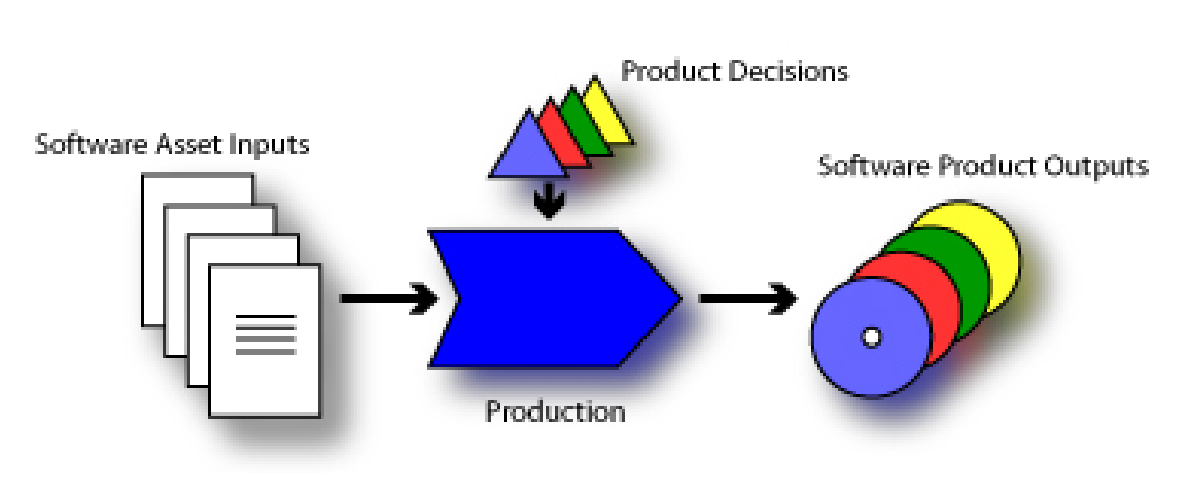
\includegraphics[scale=0.25]{img/spl.eps}\footnote{Charles W. Krueger, New
%  methods in software product line practice, CACM (2006)} 
%  }
% 
% \end{frame}

\begin{frame}
\frametitle{Thesis context}

\begin{block}{Crosscutting Nature of Variability Management}
\begin{itemize}
	\item Variable features often require variation points to be scattered
	throughout different places in requirements, design, code, and test artifacts.
\end{itemize}
\end{block}

\begin{block}{Problem}
\begin{itemize}
  \item It is hard to evolve a software product line without a clear separation
  between the problem space and the solution space.
	
  \item	However, several techniques for dealing with variations require 
	some kind of tangling between those models.    
\end{itemize}
\end{block}
\end{frame}

\begin{frame}
\frametitle{Thesis context}

\begin{block}{Proposed solution:}
A modeling framework for representing variability management techniques as
crosscutting mechanisms.
\begin{itemize}
  \item Not only independent models for variability management
  \item Main focus on composition processes of different models
\end{itemize}
%that consider different languages.
\end{block}

\begin{block}{Hypothesis}
A better separation between VM and software engineering
artifacts would improve:

\begin{itemize}
  \item SPL Evolvability
  \item SPL Traceability
  \item SPL Configurability
\end{itemize}
\end{block}

\end{frame}

% \begin{frame}
% \frametitle{Thesis context}
% 
% \begin{block}{Hypothesis}
% A better separation between VM and software engineering
% artifacts would improve:
% 
% \begin{itemize}
%   \item SPL Evolvability
%   \item SPL Traceability
%   \item SPL Configurability
% \end{itemize}
% \end{block}
% 
% \begin{block}{Proposed approach:}
% Enforce such a SoC by means of a \textcolor{DarkBlue}{framework} for
% modeling Variability Management as \textcolor{DarkBlue}{crosscutting
% mechanisms}.
% \end{block}
% \end{frame}
\section{Proposed approach}

\begin{frame}
\frametitle{VM as crosscutting mechanisms}

Different input models crosscut each other with respect to a SPL member
(adapted from Masuhara and Kiczales --- ECOOP 2003).

\onslide+<2>
\begin{block}{Big picture:}
\center{
 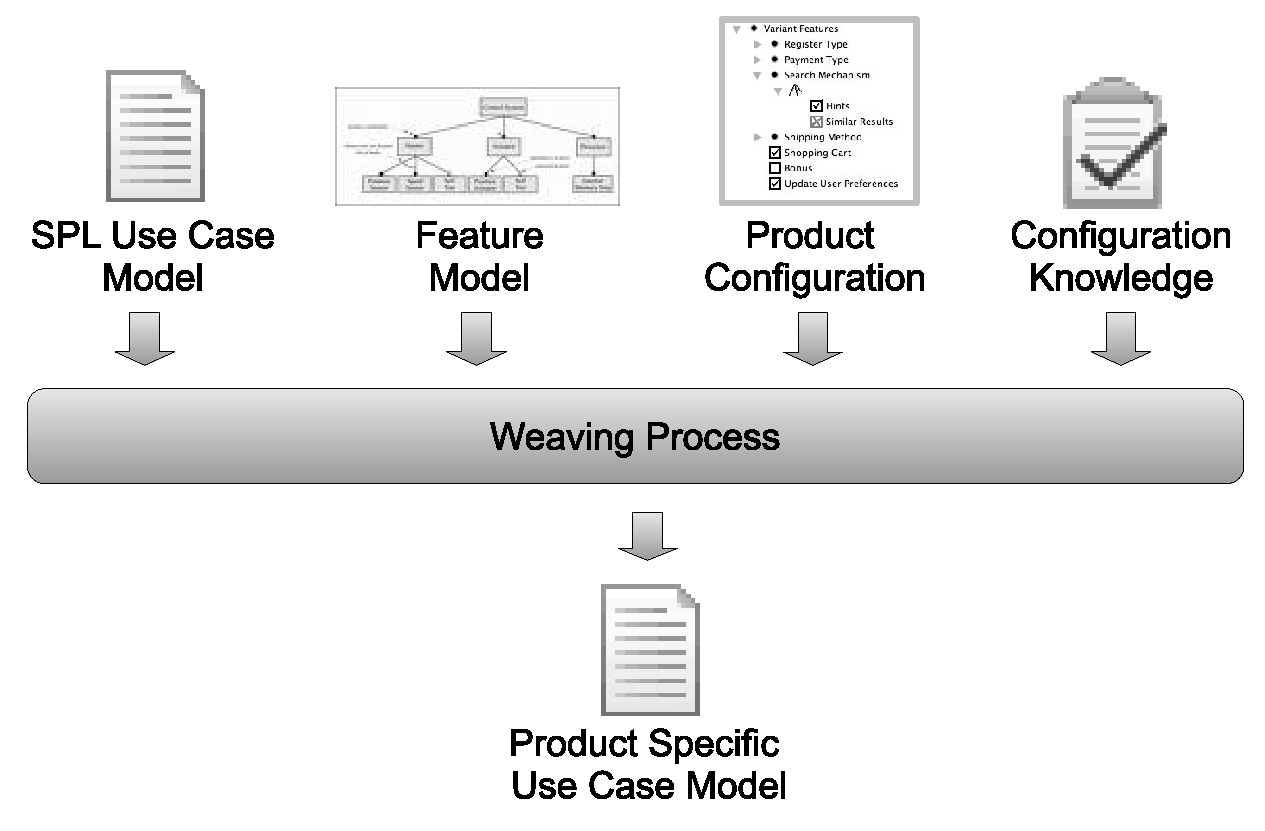
\includegraphics[scale=0.25]{img/weave-process2.eps}
}
\end{block}

\end{frame}

\begin{frame}
\frametitle{VM as crosscutting mechanisms}
\begin{block}{Weaving Process}
\begin{itemize}
  \hilite<1> \item Sequence of weavers, guided by the
  configuration knowledge, that should be applied in order to generate specific instances.
  \hilite<2> \item Each weaver is represented as a
  tuple, highlighting the contribution of the
  corresponding input languages. \\ 
  $Weaver = \{O,\ O_{VP},\ L,\ L(l)_{id},\
  	L(l)_{eff}\}$
\hilite<3> \item We depict that a weaver is
  	realizable by relating the corresponding tuple elements to a reference implementation of the weaver.
\end{itemize}	
\end{block}

\end{frame}

\begin{frame}
\frametitle{Exemplo}
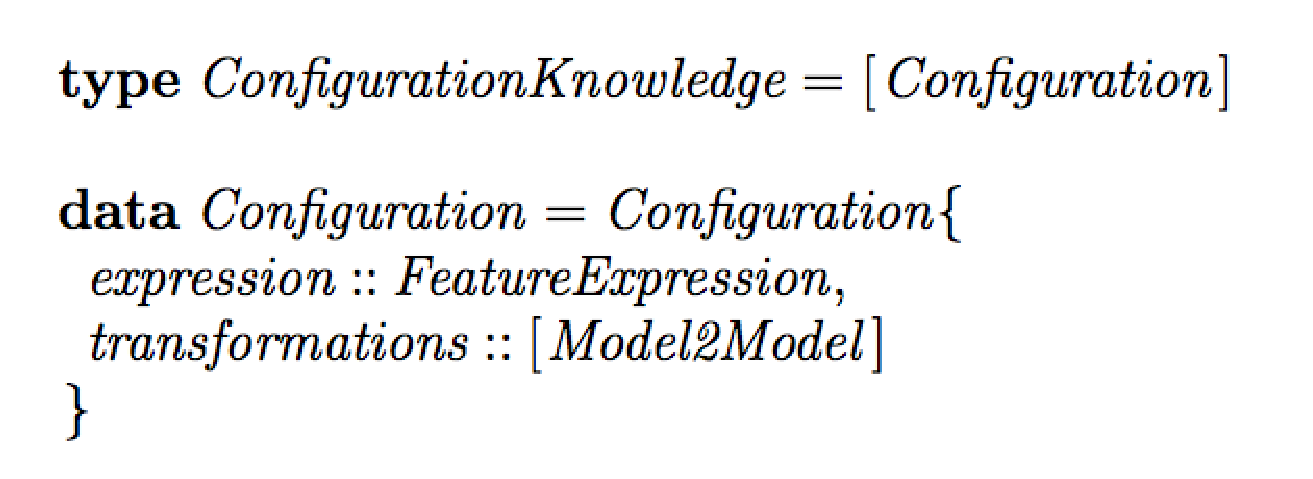
\includegraphics[scale=0.55]{img/ck.eps}
\end{frame}

\begin{frame}
\frametitle{VM as crosscutting mechanisms}
\begin{block}{Configuration knowledge}

\begin{itemize}
  \item A sequence of the algebraic data type: \textcolor{DarkBlue}{(Feature
  Expression, [Weaver])}
  \item The weaving process evaluate each feature expression. If it holds true
  for a SPL's member, the corresponding weavers are applied.
\end{itemize}
\end{block}
\center{

}
\hyperlink{ck}{\beamerbutton{code}}
\end{frame}

\begin{frame}
\frametitle{VM as crosscutting mechanisms}

\begin{center}
\begin{columns}
\begin{column}{0.4\textwidth}
 \includegraphics[scale=0.40]{img/product-line.eps}
\end{column}
\begin{column}{0.4\textwidth}
 
\end{column}
\end{columns}
\end{center}

\onslide+<2>
\begin{block}{Example of configuration knowledge}
\begin{scriptsize}
\begin{center}
\begin{tabular}{\ensuremath{\Varid{p}\{\mskip1.5mu \mathrm{1.0}\;\mathbf{in}\;\mskip1.5mu\}\Varid{p}\{\mskip1.5mu \mathrm{1.8}\;\mathbf{in}\;\mskip1.5mu\}}}
\hline 
Feature Expression &  Weavers 						\\ \hline
F1 				&  	select(square, WHITE)		\\ \hline
not(F1)			&	select(square, BLACK)		\\ \hline
F2 				&	select(circle)				\\ \hline
F2 and F3		& 	select(triangle), fill(circle, BLUE)\\ \hline				
\end{tabular}
\end{center}
\end{scriptsize}
\end{block}

\begin{block}{Example of SPL's member: $FC\ =\ (F1, F2, F3) $}
\end{block}

\end{frame}


\begin{frame}
\frametitle{VM as crosscutting mechanisms}

\begin{center}
\begin{columns}
\begin{column}{0.4\textwidth}
 \includegraphics[scale=0.40]{img/product-line.eps}
\end{column}
\begin{column}{0.4\textwidth}
 
\includegraphics[scale=0.40]{img/instance-1.eps}
\end{column}
\end{columns}
\end{center}

\begin{block}{Example of configuration knowledge}
\begin{scriptsize}
\begin{center}
\begin{tabular}{\ensuremath{\Varid{p}\{\mskip1.5mu \mathrm{1.0}\;\mathbf{in}\;\mskip1.5mu\}\Varid{p}\{\mskip1.5mu \mathrm{1.8}\;\mathbf{in}\;\mskip1.5mu\}}}
\hline 
Feature Expression &  Weavers \\ \hline
\textcolor{DarkBlue}{F1} &  \textcolor{DarkBlue}{select(square, WHITE)} \\
\hline not(F1)			&	select(square, BLACK)		\\ \hline
F2 				&	select(circle)				\\ \hline
F2 and F3		& 	select(triangle), fill(circle, BLUE)\\ \hline				
\end{tabular}
\end{center}
\end{scriptsize}
\end{block}

\begin{block}{Example of SPL's member: $FC\ =\ (F1, F2, F3) $}
\end{block}

\end{frame}

\begin{frame}
\frametitle{VM as crosscutting mechanisms}

\begin{center}
\begin{columns}
\begin{column}{0.4\textwidth}
 \includegraphics[scale=0.40]{img/product-line.eps}
\end{column}
\begin{column}{0.4\textwidth}
 
\includegraphics[scale=0.40]{img/instance-1.eps}
\end{column}
\end{columns}
\end{center}

\begin{block}{Example of configuration knowledge}
\begin{scriptsize}
\begin{center}
\begin{tabular}{\ensuremath{\Varid{p}\{\mskip1.5mu \mathrm{1.0}\;\mathbf{in}\;\mskip1.5mu\}\Varid{p}\{\mskip1.5mu \mathrm{1.8}\;\mathbf{in}\;\mskip1.5mu\}}}
\hline 
Feature Expression &  Weavers \\ \hline
\textcolor{DarkBlue}{F1} &  \textcolor{DarkBlue}{select(square, WHITE)} \\
\hline \textcolor{DarkRed}{not(F1)} & \textcolor{DarkRed}{select(square, BLACK)}\\ \hline 
F2 				&	select(circle)				\\ \hline 
F2 and F3		& 	select(triangle), fill(circle, BLUE)\\ \hline				
\end{tabular}
\end{center}
\end{scriptsize}
\end{block}

\begin{block}{Example of SPL's member: $FC\ =\ (F1, F2, F3) $}
\end{block}

\end{frame}

\begin{frame}
\frametitle{VM as crosscutting mechanisms}

\begin{center}
\begin{columns}
\begin{column}{0.4\textwidth}
 \includegraphics[scale=0.40]{img/product-line.eps}
\end{column}
\begin{column}{0.4\textwidth}
 \includegraphics[scale=0.40]{img/instance-2.eps}
\end{column}
\end{columns}
\end{center}

\begin{block}{Example of configuration knowledge}
\begin{scriptsize}
\begin{center}
\begin{tabular}{\ensuremath{\Varid{p}\{\mskip1.5mu \mathrm{1.0}\;\mathbf{in}\;\mskip1.5mu\}\Varid{p}\{\mskip1.5mu \mathrm{1.8}\;\mathbf{in}\;\mskip1.5mu\}}}
\hline 
Feature Expression &  Weavers \\ \hline
\textcolor{DarkBlue}{F1} &  \textcolor{DarkBlue}{select(square, WHITE)} \\
\hline \textcolor{DarkRed}{not(F1)} & \textcolor{DarkRed}{select(square, BLACK)}\\ \hline 
\textcolor{DarkBlue}{F2} & \textcolor{DarkBlue}{select(circle)}	\\ \hline
F2 and F3		& 	select(triangle), fill(circle, BLUE)\\ \hline
\end{tabular}
\end{center}
\end{scriptsize}
\end{block}

\begin{block}{Example of SPL's member: $FC\ =\ (F1, F2, F3) $}
\end{block}

\end{frame}

\begin{frame}
\frametitle{VM as crosscutting mechanisms}

\begin{center}
\begin{columns}
\begin{column}{0.4\textwidth}
 \includegraphics[scale=0.40]{img/product-line.eps}
\end{column}
\begin{column}{0.4\textwidth}
 \includegraphics[scale=0.40]{img/instance-3.eps}
\end{column}
\end{columns}
\end{center}

\begin{block}{Example of configuration knowledge}
\begin{scriptsize}
\begin{center}
\begin{tabular}{\ensuremath{\Varid{p}\{\mskip1.5mu \mathrm{1.0}\;\mathbf{in}\;\mskip1.5mu\}\Varid{p}\{\mskip1.5mu \mathrm{1.8}\;\mathbf{in}\;\mskip1.5mu\}}}
\hline 
Feature Expression &  Weavers \\ \hline
\textcolor{DarkBlue}{F1} &  \textcolor{DarkBlue}{select(square, WHITE)} \\
\hline \textcolor{DarkRed}{not(F1)} & \textcolor{DarkRed}{select(square, BLACK)}\\ \hline 
\textcolor{DarkBlue}{F2} & \textcolor{DarkBlue}{select(circle)}	\\ \hline
\textcolor{DarkBlue}{F2 and F3}		& 	\textcolor{DarkBlue}{select(triangle)},
fill(circle, BLUE)\\ \hline
\end{tabular}
\end{center}
\end{scriptsize}
\end{block}

\begin{block}{Example of SPL's member: $FC\ =\ (F1, F2, F3) $}
\end{block}

\end{frame}

\begin{frame}
\frametitle{VM as crosscutting mechanisms}

\begin{center}
\begin{columns}
\begin{column}{0.4\textwidth}
 \includegraphics[scale=0.40]{img/product-line.eps}
\end{column}
\begin{column}{0.4\textwidth}
 \includegraphics[scale=0.40]{img/instance-4.eps}
\end{column}
\end{columns}
\end{center}

\begin{block}{Example of configuration knowledge}
\begin{scriptsize}
\begin{center}
\begin{tabular}{\ensuremath{\Varid{p}\{\mskip1.5mu \mathrm{1.0}\;\mathbf{in}\;\mskip1.5mu\}\Varid{p}\{\mskip1.5mu \mathrm{1.8}\;\mathbf{in}\;\mskip1.5mu\}}}
\hline 
Feature Expression &  Weavers \\ \hline
\textcolor{DarkBlue}{F1} &  \textcolor{DarkBlue}{select(square, WHITE)} \\
\hline \textcolor{DarkRed}{not(F1)} & \textcolor{DarkRed}{select(square, BLACK)}\\ \hline 
\textcolor{DarkBlue}{F2} & \textcolor{DarkBlue}{select(circle)}	\\ \hline
\textcolor{DarkBlue}{F2 and F3}		& 	\textcolor{DarkBlue}{select(triangle)},
\textcolor{DarkBlue}{fill(circle, BLUE)}\\ \hline
\end{tabular}
\end{center}
\end{scriptsize}
\end{block}

\begin{block}{Example of SPL's member: $FC\ =\ (F1, F2, F3)$} \hyperlink{wp}{\beamerbutton{code}}
\end{block}

\end{frame}


\section{Modeling framework instance}

\begin{frame}
\frametitle{Walk through an example\ldots}
\onslide+<2>
\begin{block}{Environment}
\begin{itemize}
  \item VM in SPL specifications (use case scenarios)

  \begin{itemize} 
    \item Variability in function
    \item Variability in data
    \item Variability in control flow
  \end{itemize}
  \item Smart Home produtct line
\end{itemize}
\end{block}

\end{frame}

\begin{frame}
\frametitle{Variability in function}
Certain use cases and scenarios of the Smart Home PL might exist in some
products and not in others.

\begin{block}{Examples}
\begin{scriptsize}
\begin{center}
\begin{tabular}{\ensuremath{\Varid{p}\{\mskip1.5mu \mathrm{1.6}\;\mathbf{in}\;\mskip1.5mu\}\Varid{p}\{\mskip1.5mu \mathrm{0.4}\;\mathbf{in}\;\mskip1.5mu\}\Varid{p}\{\mskip1.5mu \mathrm{1.6}\;\mathbf{in}\;\mskip1.5mu\}}}
\hline 
Artifact &  & Feature \\ \hline
Configure Access to Environment & requires & Specific Environment\\ \hline
Handle Fire Detection & requires & Fire Detection \\ \hline
Notify Fire Control System & requires & Fire Detection and Control System \\ \hline
\ldots & & \ldots \\
\hline
\end{tabular}
\end{center}
\end{scriptsize}
\end{block}

\end{frame}

\begin{frame}
\frametitle{Variability in function}
\begin{center}
\includegraphics[scale=0.40]{img/select-weaver.eps}
\end{center}
\hyperlink{addScenario-weaver}{\beamerbutton{code}}
\end{frame}

\begin{frame}
\frametitle{Variability in function}
\begin{block}{Add Scenario representation }
\begin{scriptsize}
\begin{tabular}{p{0.6in}p{2.4in}}
   \hline\noalign{\smallskip}
  {\bf Element} & {\bf Description} \\
   \noalign{\smallskip}
   \hline
   \noalign{\smallskip}
   $O$             	& Scenarios of a product intance (list of scenarios) \\ 
   $O_{VP}$        	& Scenario declarations \\ 
   $L$             	& \{UCM, CK, FC\} \\ 
   $UCM_{ID}$ 	   	& IDs of the SPL scenarios \\ 
   $CK_{ID}$    	& Feature expressions and scenario's IDs\\  
   $FC_{ID}$    	& IDs of the SPL features \\ 
   $UCM_{EFF}$ 		& Provides declaration of scenarios \\  
   $CK_{EFF}$    	& Relates feature expressions to weavers \\ 
   $FC_{EFF}$    	& Selects the scenarios to be added \\
   \hline
  \end{tabular}
\end{scriptsize}
\end{block}
\end{frame}

\begin{frame}
\frametitle{Variability in data}
Certain scenarios of the Smart Home PL are parameterized.

\begin{block}{Example}
The amount of seconds to close the door depends on the product configuration.
\begin{center} 
\begin{small}
  \begin{tabular}{\ensuremath{\Varid{p}\{\mskip1.5mu \mathrm{0.2}\;\mathbf{in}\;\mskip1.5mu\}}p{1.4in}\ensuremath{\Varid{p}\{\mskip1.5mu \mathrm{1.4}\;\mathbf{in}\;\mskip1.5mu\}}}
   \hline
       Id & User Action  & System Response \\ \hline \hline
       \ldots & \ldots  & \ldots \\  \hline 
       M3 & The inhabitant informs the access password & \ldots after {\bf
       <TTC>} seconds the front door is closed \\
       \hline
    \end{tabular}
\end{small}
\end{center}
\end{block}
\end{frame}

\begin{frame}
\frametitle{Variability in data}
\begin{center}
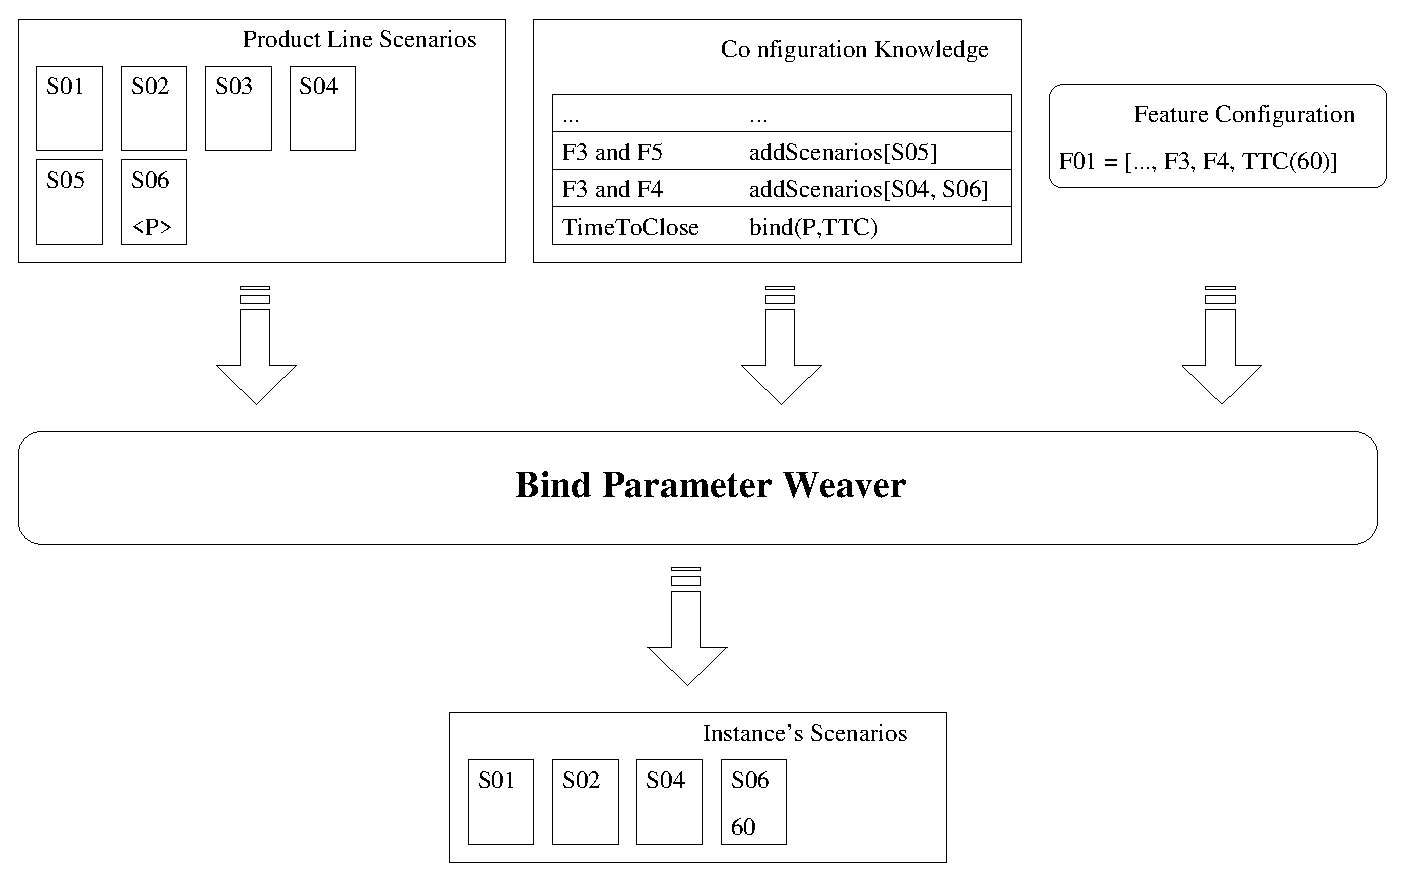
\includegraphics[scale=0.40]{img/bind-weaver.eps}
\end{center}
\end{frame}

\begin{frame}
\frametitle{Variability in data}
\begin{block}{Bind Parameter representation}
\begin{scriptsize}
\begin{tabular}{p{0.6in}p{2.4in}}
   \hline\noalign{\smallskip}
  {\bf Element} & {\bf Description} \\
   \noalign{\smallskip}
   \hline
   \noalign{\smallskip}
   $O$             	& Scenarios of a product intance (list of scenarios) \\ 
   $O_{VP}$        	& Steps of scnarios \\ 
   $L$             	& \{UCM, CK, FC\} \\ 
   $UCM_{ID}$ 	   	& Parameters declaration \\ 
   $CK_{ID}$    	& Feature expressions and parameters name\\  
   $FC_{ID}$    	& IDs of the SPL features \\ 
   $UCM_{EFF}$ 		& Provides declaration of parameterized scenarios \\  
   $CK_{EFF}$    	& Relates feature expressions to weavers \\ 
   $FC_{EFF}$    	& States the actual values of parameters \\
   \hline
  \end{tabular}
\end{scriptsize}
\end{block}
\end{frame}

\begin{frame}
\frametitle{Variability in control flow}
Certain scenarios of the Smart Home PL describe different behavior 
dependend on the product configuration.

\begin{block}{Example}
Register Inhabitant scenario varies dependend on the security mechanism that
was selected.
\end{block}
\onslide+<2>
\begin{block}{Security Mechanism = Password}
\begin{center} 
\begin{tiny}
  \begin{tabular}{\ensuremath{\Varid{p}\{\mskip1.5mu \mathrm{0.2}\;\mathbf{in}\;\mskip1.5mu\}}p{1.8in}\ensuremath{\Varid{p}\{\mskip1.5mu \mathrm{1.8}\;\mathbf{in}\;\mskip1.5mu\}}}
   \hline
       Id & User Action  & System Response \\ \hline \hline
       M1 & \ldots.  & \ldots \\  \hline
       
       P1 & The home owner fills in the inhabitant personal form and selects
       the proceed option. & The system requires the inhabitant password (and password
       confirmation) for getting access to the home. \\ \hline 
       
       P2 & The new inhabitant fills in the password (and confirmation
       password) for home access. & The system requests the home owner
       configuration password. \\
       \hline
       
       M2 & \ldots.  & \ldots \\  \hline
    \end{tabular}
\end{tiny}
\end{center}
\end{block}
\end{frame}

\begin{frame}
\frametitle{Variability in control flow}
Certain scenarios of the Smart Home PL describe different behavior 
dependend on the product configuration.

\begin{block}{Example}
Register Inhabitant scenario varies dependend on the security mechanism that
was selected.
\end{block}
\begin{block}{Security Mechanism = Finger Print}
\begin{center} 
\begin{tiny}
  \begin{tabular}{\ensuremath{\Varid{p}\{\mskip1.5mu \mathrm{0.2}\;\mathbf{in}\;\mskip1.5mu\}}p{1.8in}\ensuremath{\Varid{p}\{\mskip1.5mu \mathrm{1.8}\;\mathbf{in}\;\mskip1.5mu\}}}
   \hline
       Id & User Action  & System Response \\ \hline \hline
       M1 & \ldots.  & \ldots \\  \hline
       
       F1 & The home owner fills in the inhabitant personal form and selects
       the proceed option. & The system requires the inhabitant inhabitant finger print to capture it. \\ \hline 
       
       F2 & The new inhabitant put his finger in the finger print capture
       device. & The system requests the home owner configuration password. \\
       \hline
       
       M2 & \ldots.  & \ldots \\  \hline
  \end{tabular}
\end{tiny}
\end{center}
\end{block}
\end{frame}

\begin{frame}
\frametitle{Variability in control flow}
\begin{center}
\includegraphics[scale=0.40]{img/aspect-weaver.eps}
\end{center}
\hyperlink{aspect-code}{\beamerbutton{code}}
\end{frame}

\begin{frame}
\frametitle{Variability in data}
\begin{block}{Evaluate Aspect representation}
\begin{scriptsize}
\begin{tabular}{p{0.6in}p{2.4in}}
   \hline\noalign{\smallskip}
  {\bf Element} & {\bf Description} \\
   \noalign{\smallskip}
   \hline
   \noalign{\smallskip}
   $O$             	& Scenarios of a product intance (list of scenarios) \\
   $O_{VP}$        	& Steps of scnarios \\
   $L$             	& \{AUCM, UCM, CK, FC\} \\
   $AUCM_{ID}$ 		& Step ids or step annotations \\
   $UCM_{ID}$ 		& Scenario declaration \\
   $CK_{ID}$    	& Feature expressions and aspects name\\
   $FC_{ID}$    	& IDs of the SPL features \\
   $AUCM_{EFF}$ 	& Augments scenario specifications	\\
   $UCM_{EFF}$ 		& Provides declaration of scenarios \\
   $CK_{EFF}$    	& Relates feature expressions to weavers \\
   $FC_{EFF}$    	& Selects the aspects to be evaluated \\
   \hline
  \end{tabular}
\end{scriptsize}
\end{block}
\end{frame}

\section{Concluding remarks}

\begin{frame}
\frametitle{Concluding remarks and future work}
\begin{block}{Contributions}
\begin{itemize}
  \item A novel approach for representing VM 
  \item New techniques proposed for VM in use case scenarios
  \item A Haskell DSL for variability management
  \begin{itemize}
    \item Feature modeling (integrated to FM Plugin)
    \item Product generation
  \end{itemize}  
  \item A suite of metrics adapted to our research context
\end{itemize}
\end{block}

\end{frame}

\begin{frame}
\frametitle{Concluding remarks and future work}
\begin{block}{Evaluation}
\begin{itemize}
  \item We have evaluated our proposals in three case studies, and observed: 
  \begin{itemize}
    \item A reduction in the size of specifications
    \item Features better modularized (DOS, DOF) 
    \item Improvements in SPL evolvability
  \end{itemize}  
\end{itemize}
\end{block}

\end{frame}

\begin{frame}
\frametitle{Concluding remarks and future work}
\begin{block}{Next steps}
\begin{itemize}
  \item Plan and execute a controlled experiment 
  \item Instantiate the modeling framework to other types of artifacts  
  \item Release a version of our Haskell Libraries and tools
\end{itemize}
\end{block}

\end{frame}

\begin{frame}
\titlepage
\end{frame}

\section*{Backup}

\begin{frame}[fragile]
\frametitle{Code Generation}

\begin{block}{velocity}
\end{block}
\begin{small}
\begin{tabbing}\tt
~public~interface~Expression~\char123{}\\
\tt ~~~~~~~~~public~\char36{}type~eval\char40{}\char41{}\char59{}\\
\tt ~\char35{}if\char40{}\char36{}print\char41{}\\
\tt ~~~~~~~~~public~String~print\char40{}\char41{}\char59{}\\
\tt ~\char35{}end\\
\tt ~\char125{}
\end{tabbing}
\end{small}
\end{frame}

\begin{frame}[fragile]
\frametitle{Code Generation}

\begin{block}{velocity}
\end{block}
\begin{small}
\begin{tabbing}\tt
~public~class~BinaryExp~implements~Expression~\char123{}\\
\tt ~~~~~~~~~\char46{}\char46{}\char46{}\\
\tt ~~~~~~~~~public~String~getOperator\char40{}\char41{}~\char123{}\\
\tt ~~~~~~~~~~~~~~~~~return~operator\char59{}\\
\tt ~~~~~~~~~\char125{}\\
\tt ~~~~~~~~~\\
\tt ~\char35{}if\char40{}\char36{}print\char41{}\\
\tt ~~~~~~~~~public~String~print\char40{}\char41{}~\char123{}\\
\tt ~~~~~~~~~~~~~~~~~return~left\char46{}print\char40{}\char41{}~\char43{}~operator~\char43{}~right\char46{}print\char40{}\char41{}\char59{}\\
\tt ~~~~~~~~~\char125{}\\
\tt ~\char35{}end\\
\tt ~\char125{}
\end{tabbing}
\end{small}
\end{frame}



\begin{frame}
\frametitle{Message Application Product Line}

\begin{block}{Feature model}
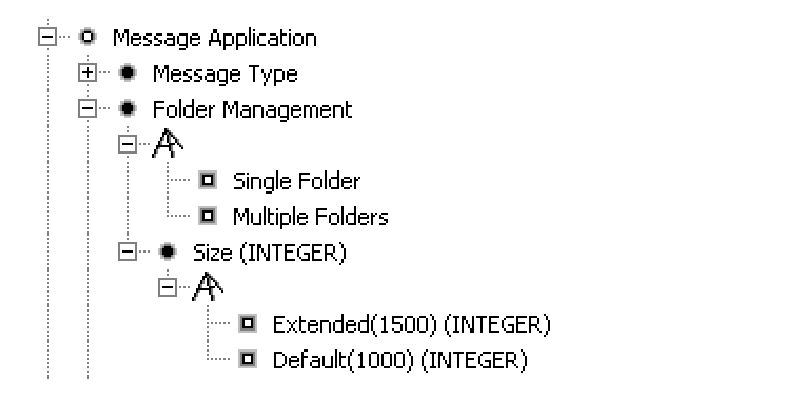
\includegraphics[scale=0.5]{img/fm03.eps}
\end{block}
\end{frame}

\begin{frame}
\frametitle{PLUC Notation}
\begin{block}{No separation between VM and software assets}
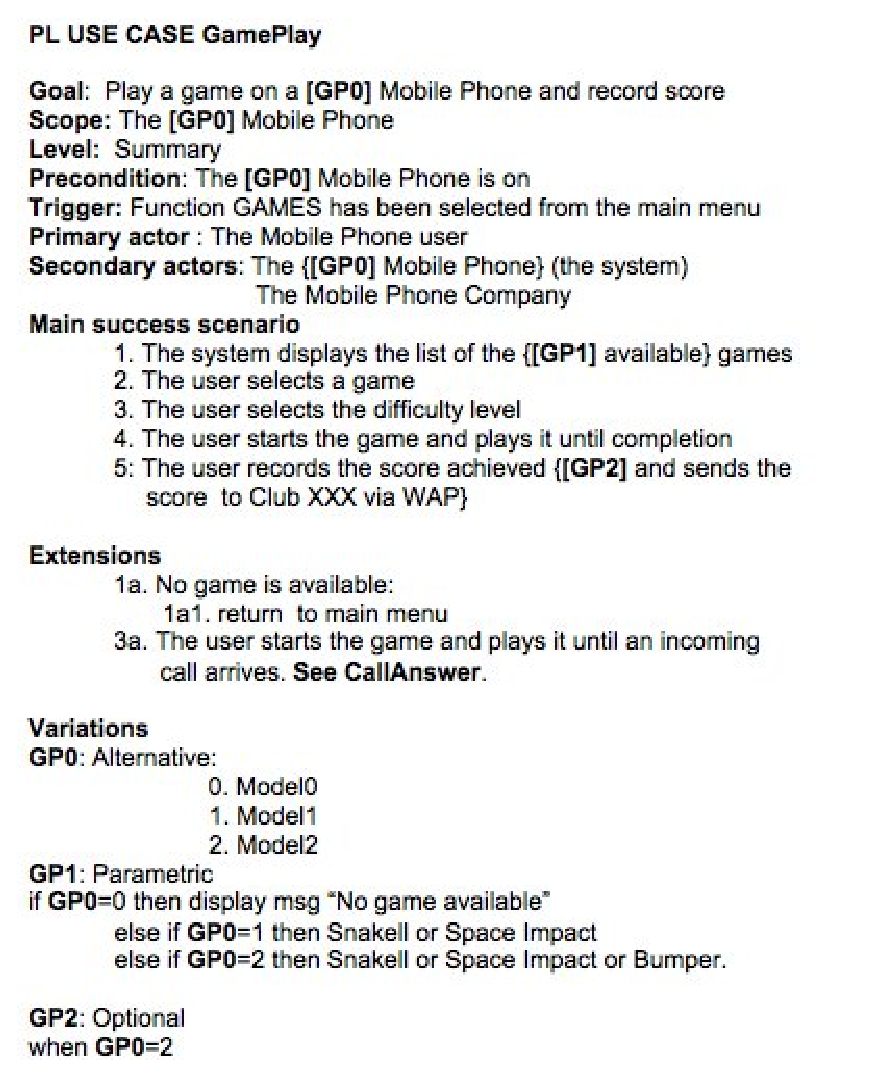
\includegraphics[scale=0.4]{img/pluc.eps}
\end{block}
\end{frame}

\begin{frame}[fragile,label=ck]
\frametitle{Configuration Knowledge}
\begin{block}{Abstract Syntax}
\begin{center}
\begin{tiny}
\begin{lstlisting}[frame=tb]
type ConfigurationKnowledge = [Configuration]
 
data Configuration  = Configuration {
 expression :: FeatureExpression,
 weavers :: [Model2Model] 	 
}
\end{lstlisting}
\end{tiny}
\end{center}
\end{block}
\end{frame}

\begin{frame}[fragile,label=wp]
\frametitle{Configuration Knowledge}

\begin{block}{Weaving Process}
\begin{center}
\begin{tiny}
\begin{lstlisting}[frame=tb]

buildConfiguration spl fc ck = applyAllTransformations spl ck (emptyInstance spl fc)
    
applyAllTransformations spl [] productInstance = productInstance
applyAllTransformations spl (x:xs) productInstance = 
 let
 	f = (instanceConfiguration productInstance)
 	e = (expression x) 
 	w = (weavers x)
   in if (eval f e) 
      then applyAllTransformations spl xs (applyTransformations spl w productInstance) 
      else applyAllTransformations spl xs productInstance
\end{lstlisting}
\end{tiny}   
\end{center}  
\end{block}

\end{frame}

\begin{frame}[fragile,label=addScenario-weaver]
\frametitle{Reference Implementations}

\begin{block}{Add Scenario}
\begin{center}
\begin{tiny}
\begin{lstlisting}[frame=tb]

addScenariosM2M :: [Id] -> ProductLine -> ProductInstance -> ProductInstance
addScenariosM2M ids spl productInstance =
 let
 	inputUCM = splUseCaseModel spl
 	outputUCM = instanceUseCaseModel productInstance
	ins = ucmScenarios inputUCM
	outUseCases = useCases outputUCM
	rName = ucmName outputUCM
	rUseCases = addUseCaseM2M inputUCM outputUCM  [s \ensuremath{\Varid{s}\leftarrow \Varid{ins},\Varid{exists}\;(\Varid{scenarioId}\;\Varid{s})\;\Varid{ids}\mskip1.5mu]\;\Varid{rAspects}\mathrel{=}\Varid{aspects}\;\Varid{outputUCM}\;\mathbf{in}\;\Varid{productInstance}\{\mskip1.5mu \Varid{instanceUseCaseModel}\mathrel{=}\Conid{UCM}\;\Varid{rName}\;\Varid{rUseCases}\;\Varid{rAspects}\mskip1.5mu\}\lambda \Varid{end}\{\mskip1.5mu \Varid{lstlisting}\mskip1.5mu\}\lambda \Varid{end}\{\mskip1.5mu \Varid{tiny}\mskip1.5mu\}\lambda \Varid{end}\{\mskip1.5mu \Varid{center}\mskip1.5mu\}\lambda \Varid{end}\{\mskip1.5mu \Varid{block}\mskip1.5mu\}\lambda \Varid{end}\{\mskip1.5mu \Varid{frame}\mskip1.5mu\}\lambda \Varid{begin}\{\mskip1.5mu \Varid{frame}\mskip1.5mu\}[\mskip1.5mu \Varid{fragile},\Varid{label}\mathrel{=}\Varid{aspect}\mathbin{-}\Varid{code}\mskip1.5mu]\lambda \Varid{frametitle}\{\mskip1.5mu \Conid{Aspectual}\;\Conid{Use}\;\Conid{Case}\mskip1.5mu\}\lambda \Varid{begin}\{\mskip1.5mu \Varid{block}\mskip1.5mu\}\{\mskip1.5mu \Conid{Abstract}\;\Conid{Syntax}\mskip1.5mu\}\lambda \Varid{begin}\{\mskip1.5mu \Varid{center}\mskip1.5mu\}\lambda \Varid{begin}\{\mskip1.5mu \Varid{tiny}\mskip1.5mu\}\lambda \Varid{begin}\{\mskip1.5mu \Varid{lstlisting}\mskip1.5mu\}[\mskip1.5mu \Varid{frame}\mathrel{=}\Varid{tb}\mskip1.5mu]\;\mathbf{data}\;\Conid{AspectualUseCase}\mathrel{=}\Conid{AspectualUseCase}\{\mskip1.5mu \Varid{aspectId}\mathbin{::}\Conid{Id},\Varid{aspectName}\mathbin{::}\Conid{Name},\Varid{advices}\mathbin{::}[\mskip1.5mu \Conid{Advice}\mskip1.5mu]\mskip1.5mu\}\;\mathbf{deriving}\;(\Conid{Show})\;\mathbf{data}\;\Conid{Advice}\mathrel{=}\Conid{BeforeAdvice}\{\mskip1.5mu \Varid{pointCut}\mathbin{::}[\mskip1.5mu \Conid{StepRef}\mskip1.5mu],\Varid{aspectualScenario}\mathbin{::}\Conid{Scenario}\mskip1.5mu\}} 
 AfterAdvice { pointCut :: [StepRef], aspectualScenario :: Scenario }

\end{lstlisting}
\end{tiny}
\end{center}
\end{block}
\end{frame}

\end{document}
